\documentclass{article} % For LaTeX2e
\usepackage{cos424,times}
\usepackage{hyperref}
\usepackage{url}
\usepackage{graphicx}
\usepackage{amsmath}
\usepackage{multirow}
\usepackage{listings}
\usepackage{float}
\lstset{frame=tb,
  language=R,
  aboveskip=3mm,
  belowskip=3mm,
  showstringspaces=false,
  columns=flexible,
  basicstyle={\small\ttfamily},
  numbers=none,
  numberstyle=\tiny\color{gray},
  keywordstyle=\color{blue},
  commentstyle=\color{dkgreen},
  stringstyle=\color{mauve},
  breaklines=true,
  breakatwhitespace=true
  tabsize=3
}
\bibliographystyle{plos2009}


\title{COS424 Assignment 1: Email Classification}


\author{
Eddie D Zhou\\
ORFE '16\\
Princeton University\\
\texttt{edzhou@princeton.edu} \\
\And
Daway Chou-Ren\\
COS '16\\
Princeton University\\
\texttt{dchouren@princeton.edu} \\
}

\newcommand{\fix}{\marginpar{FIX}}
\newcommand{\new}{\marginpar{NEW}}

\begin{document}

\maketitle

\begin{abstract}
Spam has plagued the inboxes of email users for decades now, and new companies and technologies have risen to fight the influx of ``the use of electronic messaging systems to send unsolicited messages (spam), especially advertising, as well as sending messages repeatedly on the same site.''  In this assignment, we address the problem of classifying emails into spam or ham (not spam) using two different feature sets, and a variety of different classifiers.  The datasets used are the training and testing partitions of the TREC 2007 spam track overview dataset.  We find that logistic regression in conjunction with bag-of-words features achieves the highest accuracy. but when examining different classifiers in a more refined and smaller feature space, a linear support vector machine achieves the best performance.
\end{abstract}
\section{Introduction}
According to a report on workplace productivity by McKinsey, workers spend up to 28\% of their time checking their email.  While most companies have a rigorous spam filter or secure email gateway in place (such as Proofpoint or Gmail), it is still a fruitful exercise in machine learning to examine classifier and feature extraction in the spam space.\par 
We first use the given ``vanilla'' feature extraction strict, modified to threshold 100, to extract bag-of-word features from our dataset.  Using cross-validation, we obtain a validation score for each of the following three models -- Naive Bayes, Logistic Regression, and AdaBoost.  Picking the highest validation score, we re-train the model on the full training set, and obtain the final test accuracy upon the testing set originally given.\par 
Next, as more of an experiment, we use custom features extracted with more meaning than simple bag-of-words features.  Splitting the training set into a simple training / validation partition, we train the following models on the sub-training set -- Random Forests, SVM (Gaussian), SVM (Sigmoid), SVM (Linear), Deep Neural Network, and Logistic Regression.  We take the model with the highest accuracy on the untouched validation set, and then re-train said model on the full training set.  Finally, we evaluate this model on the testing set to obtain an unbiased test accuracy.
%\section{Related Work}
%
%This data set is the canonical text multi class classification data set in the machine learning community, and has been used as a benchmark for text classification methods in many contexts. In particular, recent text classification methods have used the bag-of-words representation of this data set projected down to a set of latent \emph{topics}, where the projection is informed by the class label~\cite{zhu2009,lacoste2009}. Then, for testing, new posts also are considered in the context of the low-dimensional topic space instead of their bag-of-words representation. This suggests that feature selection may benefit the classification task.
\subsection{Data processing}
(insert description of data)\par 
The TREC 2007 dataset was downloaded from the COS424 Piazza website on February 13th, 2015, with the folder already partitioned into a 90/10 training and testing split.  Using the \lstinline{email_process.py}\lstinline{} script that was written for us (with a small modification of dictionary threshold 200 lowered to 100), we extracted enough word counts for each training and testing emai to form a dataframe with the 45000 examples, and 15228 features per email.\par 
For the custom features, we )insert stuff from Daway's explanation here)
\subsection{Classification methods}

We use three different classification methods from the SciKitLearn Python libraries for the vanilla feature set (all parameterizations are the default unless specified)
\begin{enumerate}
\item \emph{Naive Bayes} (NB): Using the default parameters of MultinomialNB()
\item \emph{Logistic regression with $\ell_2$ penalty} (LOG): built on liblinear library
\item \emph{AdaBoost} (AdB): using $50$ decision trees as weak learners
\end{enumerate}

For the custom feature set, we use six different classification methods in R:
\begin{enumerate}
\item \emph{Random Forest} (RF): default params of randomForest
\item \emph{Support Vector Machine (Gaussian)} (SVMG): default params
\item \emph{Support Vector Machine (sigmoid)} (SVMS): default params
\item \emph{Support Vector Machine (linear)} (SVML): default params
\item \emph{Deep Neural Network} (DNN): 100 epochs, tanh activation, 3 layers of 50 nodes, 50\% drop-out for each layer, 20\% of inputs dropped
\end{enumerate}
\subsection{Evaluation}
In the vanilla feature space, we used 5-fold cross validation on the full training set to obtain a full generalization error for each of the three models.  This is a simple accuracy metric -- we sum the total number of errors each model incurred on each validation fold, and subtract it from 1.  The k-fold cross validation gives us a prediction for each training sample when it is unseen, allowing us to use that total error as a metric to choose between models.  In other words, we have the metric $A_q$ for model $q$:
\begin{align*}
A_q &= 1 - \frac{\sum_{i=1}^5(FP_{fi} + FN_{fi})}{N}
\end{align*}
where $FP_{fi}$ is the number of false positives obtained from training on all folds but fold $i$, and predicting on fold $i$ (likewise for the false negatives $FN_{fi}$.\par
For our experimental custom feature set, we simply set aside 20\% of the training set as a validation set, to avoid the cost of training the same model $k$ times in the cross validation.  Here, we also obtain some more in-depth metrics rather than just the validation accuracy: we also use the precision, recall, $F_1$-score, and log loss metrics, defined as
\begin{align*}
\text{precision} &= \frac{TP}{TP + FP}\\
\text{recall} &= \frac{TP}{TP + FN}\\
F_1 &= 2 \cdot \frac{\text{precision } \cdot \text{ recall}}{\text{precision } + \text{ recall}}\\
\text{log-loss} &= -\frac{1}{N}\sum_{i=1}^N\sum_{j=1}^My_{i,j}\log(p_{i,j})
\end{align*}
where for the log-loss, there are $N$ samples, $M$ classes (2 in our case), $y_{i,j}$ is 1 if sample $i$ is in class $j$, and 0 otherwise, and $p_{i,j}$ is the model's probabilistic estimate of sample $i$ belonging in class $j$.
\section{Results}
\subsection{Evaluation results}
\subsubsection{Vanilla Features}
For our vanilla features and three models, we include the number of misclassified samples in each validation fold (indexing from f0 to f4 instead of f1 to f5), the average number of misclassifications per fold, as well as the total number of misclassifications, which is easily manipulated into the generalization error (and accuracy).
\begin{table}[h]
\centering
\large
\begin{tabular}{|c|c|c|c|c|c|c|c|c|}
\hline
    & f0 & f1 & f2 & f3 & f4 & average & total & gen\_acc \\ \hline
NB  & 29 & 18 & 21 & 38 & 25 & 26.2    & 131   & 0.997089 \\ \hline
LOG & 12 & 9  & 9  & 15 & 10 & 11.0    & 55    & 0.998778 \\ \hline
AdB & 13 & 19 & 15 & 26 & 21 & 18.8    & 94    & 0.997911 \\ \hline
\end{tabular}
\end{table}
While it's clear that the total validation accuracy is extremely high for all three methods, it is clear that the Logistic Regression model obtains the highest accuracy with respect to the entire validation process.\par 
Taking the logistic regression as our ``best model'', we re-train it on the full training set and then evaluate it in an unbiased fashion on the test set.  Doing so gives us an accuracy that is comparable to the generalization accuracy obtained during the validation phase -- \textbf{99.762\%}.  Given this extraordinarily high test accuracy, we should expect to see a relatively strange ROC curve, one that spikes up immediately as the threshold moves down from 99.99...\% to 0\%.
\begin{figure}[h]
\centering
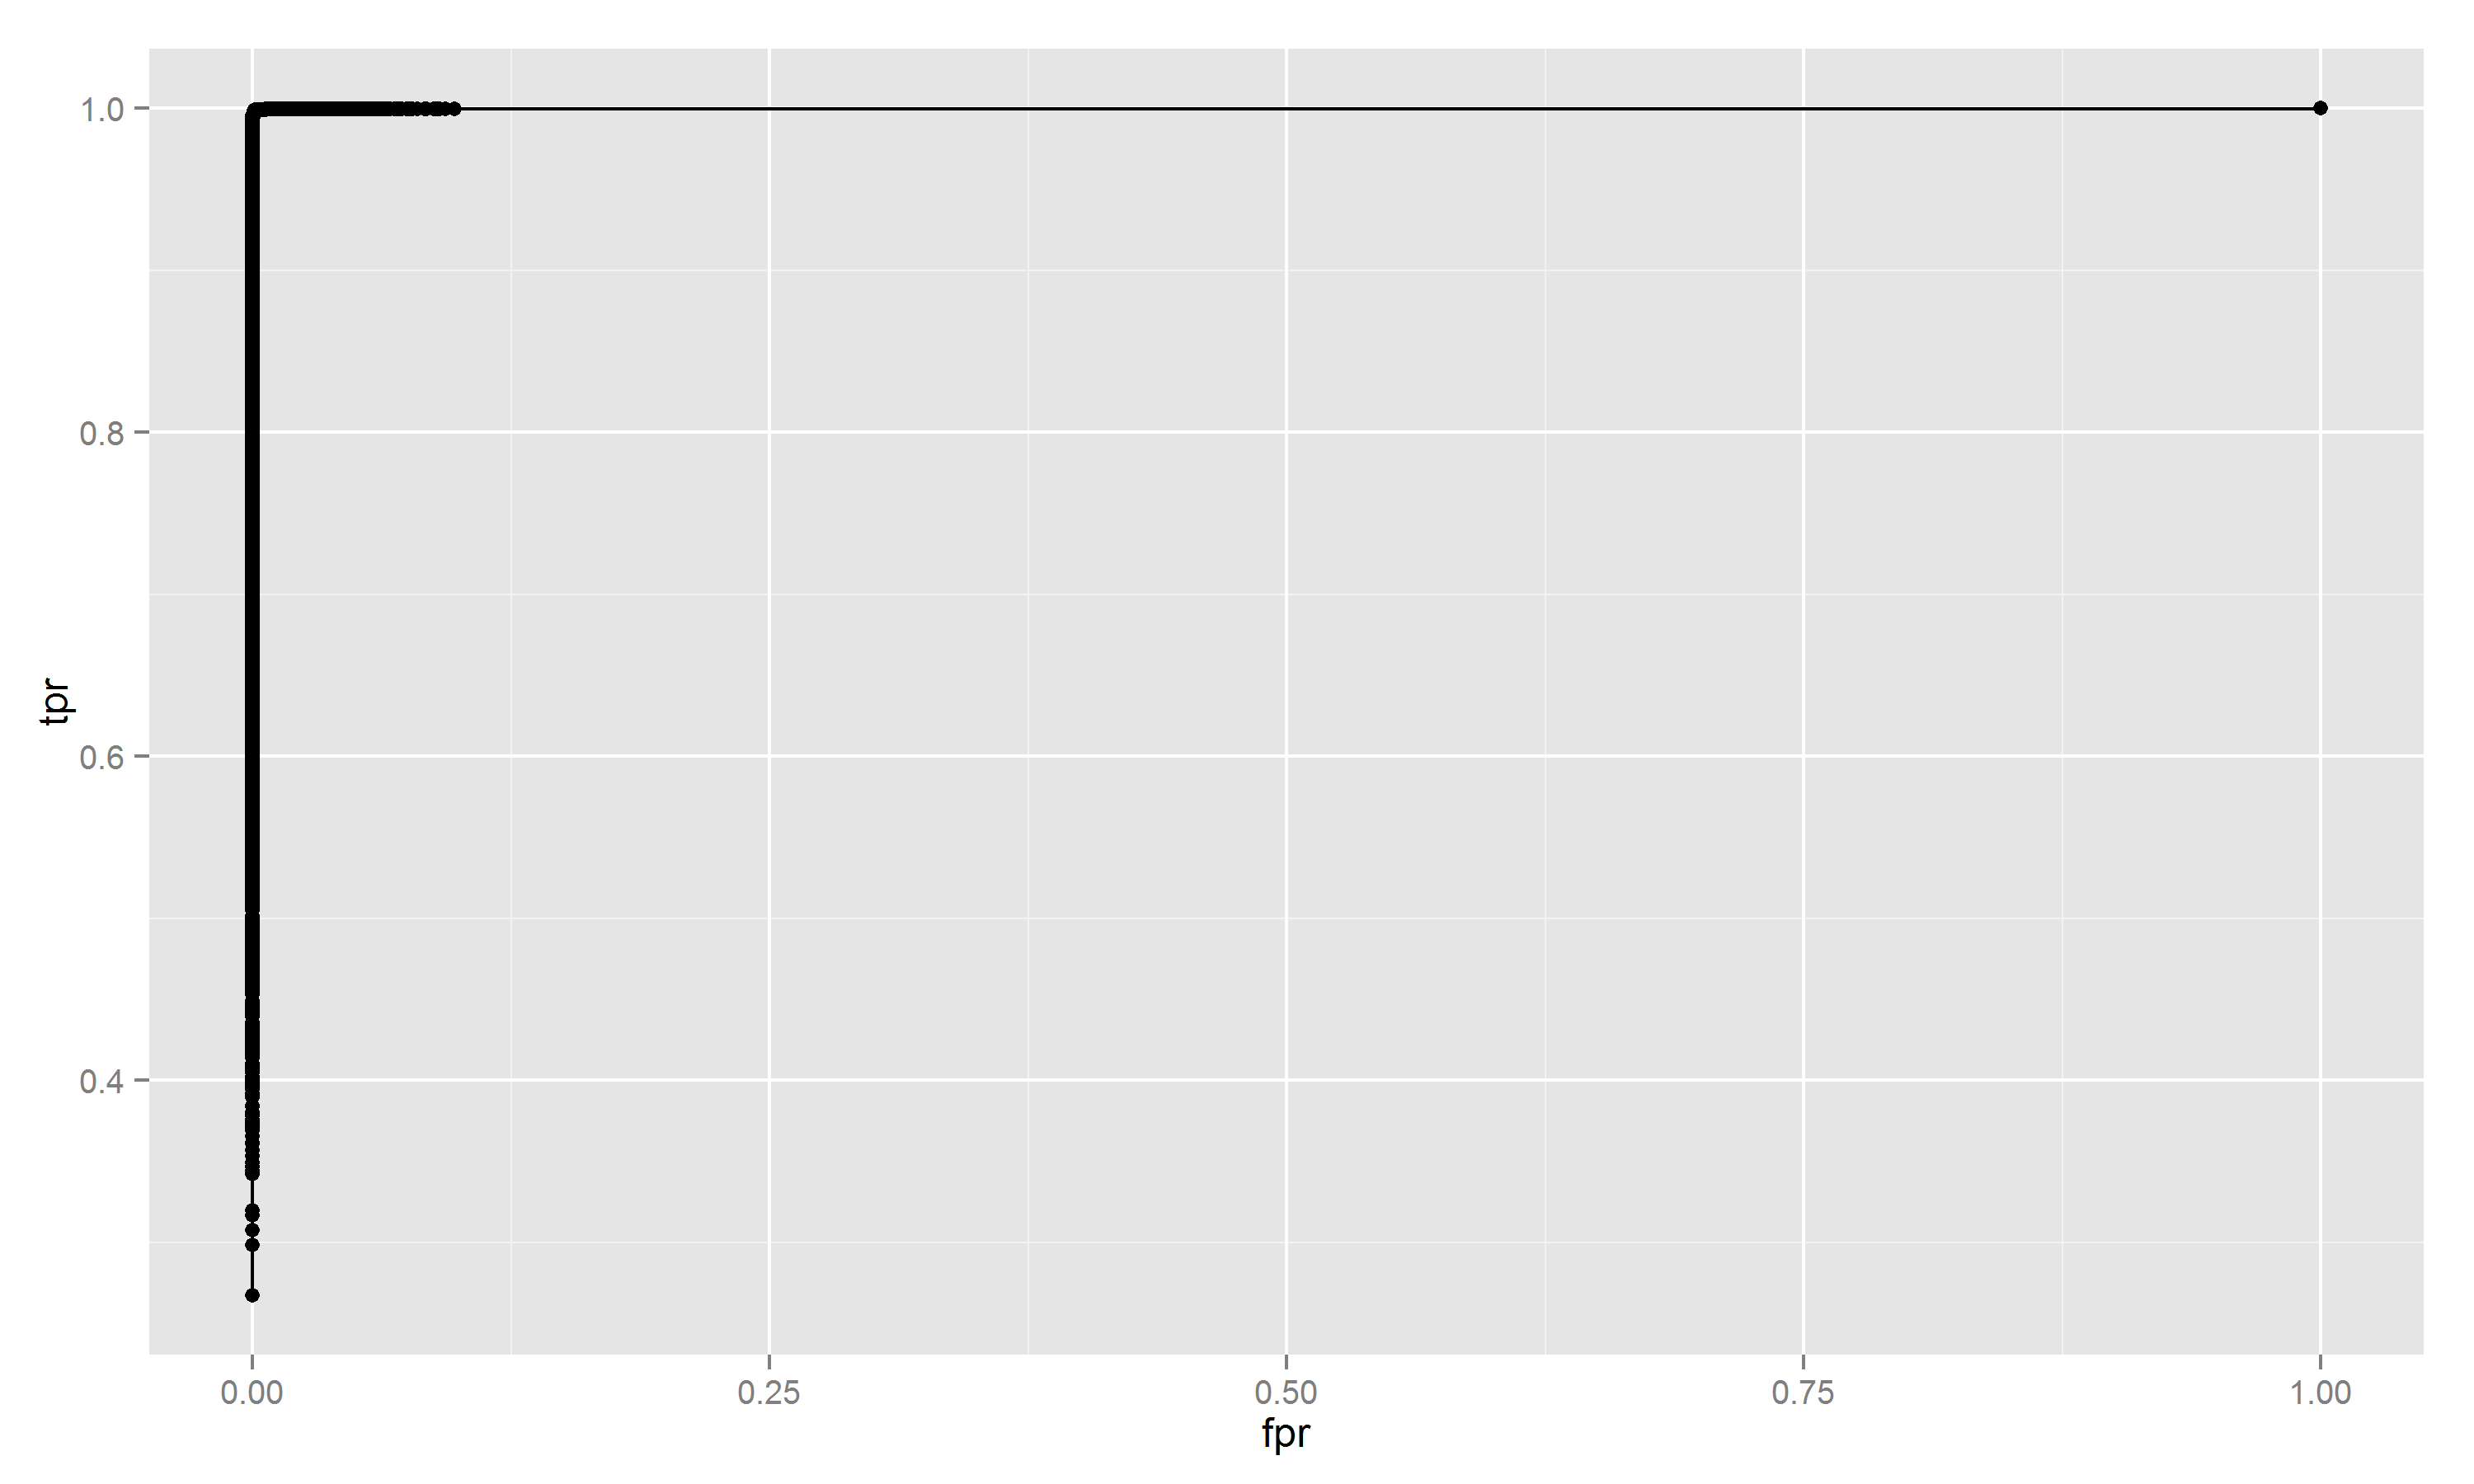
\includegraphics[width=140mm]{roc_vanilla.png}
\end{figure}
This tells us that we are near our perfectly desired $(0, 1)$ point.  This makes sense, because when we have a very high threshold, everything is classified as negative, and, as with all ROC curves, the first point is at $(0, 0)$.  But because the classifier is so strong, its predicted probabilities are very close to 0 and 1, so the threshold only needs to be relaxed a small amount before the true positive rate shoots up.  The ROC curves of such successful classifiers are almost misleading -- with the points overlaid on the curve, we see that the fpr value simply jumps from 0.09 to 1 as the threshold goes to 0.
\subsubsection{Custom Features}
Because the more refined feature space is defined by only 63 features, the classifiers are working with less data and should be expected to have lower validation and testing scores.  The idea here is that with much lower space, time, and computational costs, we might be able to achieve decent performance.
\begin{table}[H]
\centering
\begin{tabular}{|l|l|l|l|l|l|}
\hline
             & validation accuracy & log loss   & precision & recall    & $F_1$     \\ \hline
RF           & 0.5796667           & 0.3951222  & 0.8917411 & 0.1781494 & 0.2969708 \\ \hline
SVM\_gauss   & 0.4983333           & 0.1532875  & 0.4983333 & 1.0000000 & 0.6651835 \\ \hline
SVM\_sigmoid & 0.3371111           & 3.6592386  & 0.3623350 & 0.4345596 & 0.3951744 \\ \hline
SVM\_linear  & 0.8593333           & 0.6662509  & 0.8217070 & 0.9166109 & 0.8665683 \\ \hline
DNN          & 0.5195556           & 0.8806850  & 0.5176342 & 0.5268673 & 0.4307182 \\ \hline
Logistic     & 0.4610000           & 10.2988752 & 0.4563246 & 0.4263099 & 0.4493372 \\ \hline
\end{tabular}
\end{table}
It is clear that the linear support vector machine blew all of the other models out of the water, with a much higher validation accuracy, precision, recall, and $F_1$ score.  Since we have more models and computational capacity here, we also provide the ROC curves of every model on the validation set:
\begin{figure}[h]
\centering
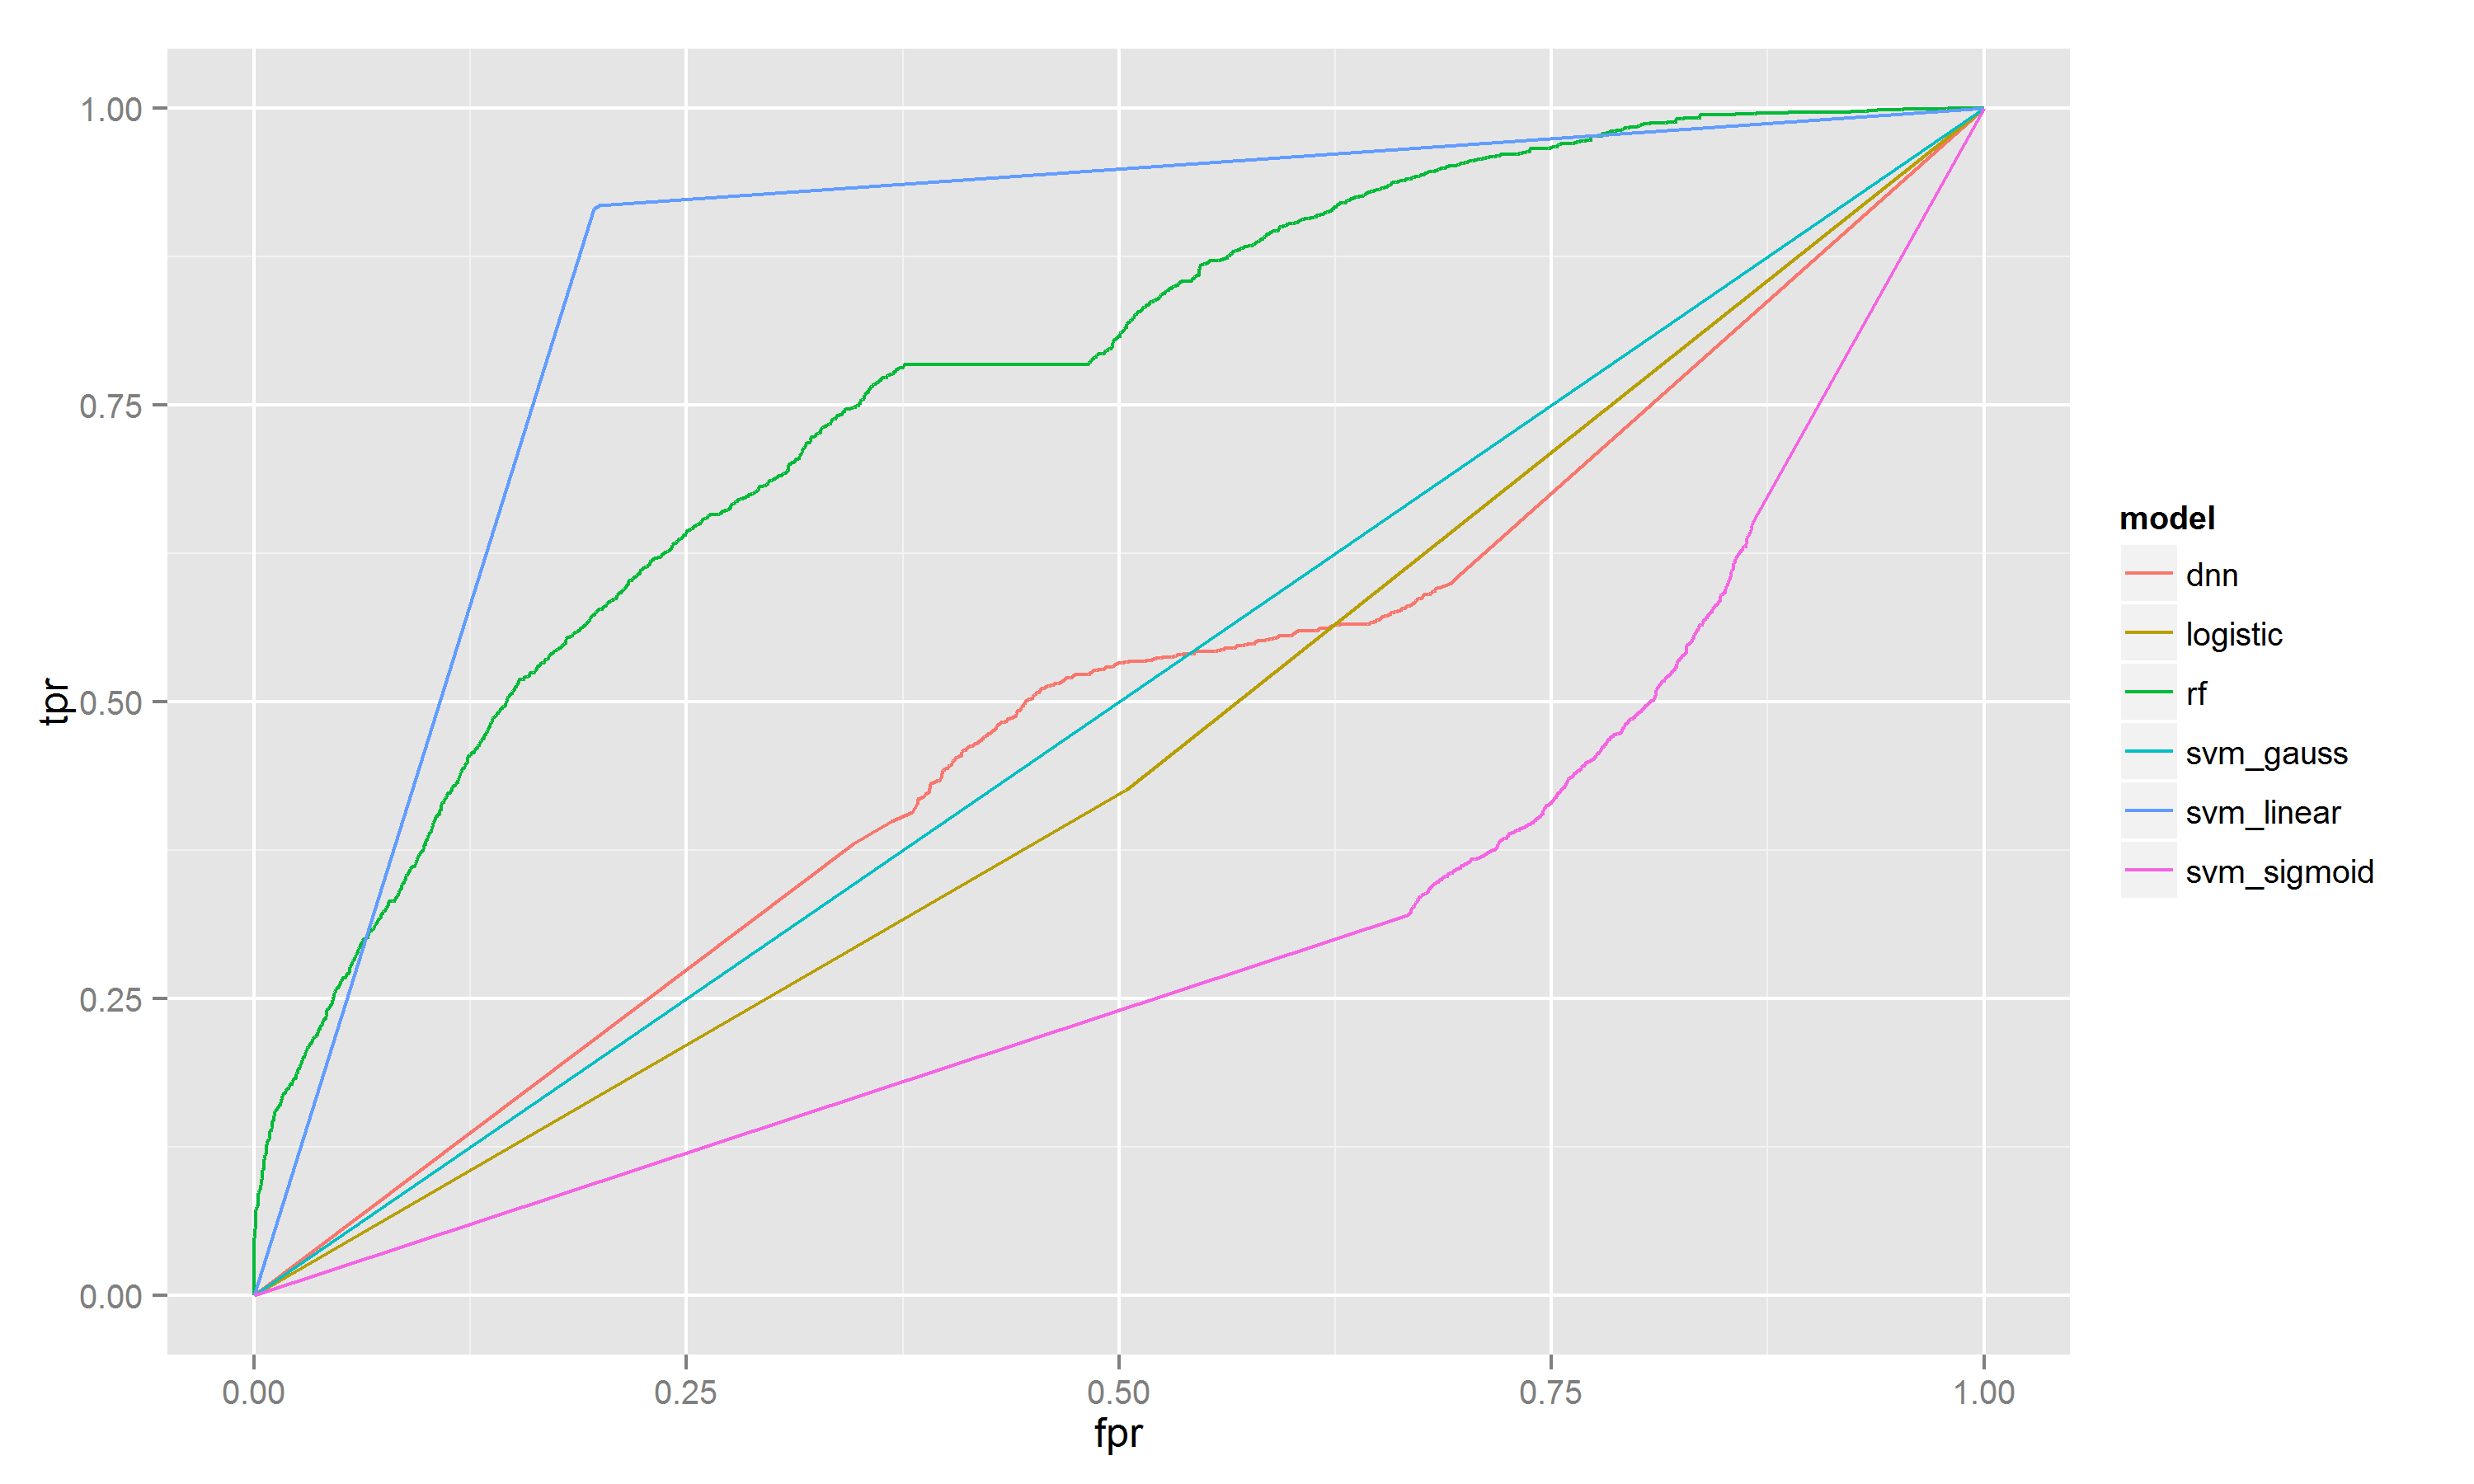
\includegraphics[width=150mm]{roc_custom.png}
\end{figure}
The ROC curves confirm the numbers, telling us that the linear support vector machine is the model to move forward with.  Re-training on the full training set, and then applying to the testing set gives us \textbf{88.98\% accuracy}, which is very comparable to the vanilla feature set, especially considering the space, time, and computational improvements.
\subsection{Computational speed}
As expected, all of the classifiers' had much shorter training times on the custom features set than the times on the higher-dimensional vanilla feature set.  Among the vanilla feature models, KNN was originally considered, but the prediction phase took too long given the massive distance calculations involved.  Of the three, Naive Bayes was quicker than the Logistic Regression, which was much quicker than AdaBoost (which requires training all the weak learner decision trees).  For the custom feature set, the support vector machines all took longer than the random forest, neural network, and logistic regression (with linear taking the longest).
\section{Discussion}
The difference in models considered in the validation phase between the vanilla and custom feature sets (as well as the choice to partition out a set validation set rather than employ cross-validation in the custom feature training) was due largely to the desire for experimentation.  The two final test accuracies are not directly compared -- in any case, given the extraordinarily high validation and test accuracies in the models trained on the vanilla feature set, there is not a large difference in performance.  This leads us to believe that even if we were to spend the huge amount of time necessary to train the linear support vector machine in 15228-space, the gain in accuracy over the more parsimonious and efficient logistic regression would be negligible.
\subsection{Vanilla}
Given the extremely high accuracy of the logistic regression on the vanilla feature datasets, it would be interesting to examine the incorrectly classified examples from that testing dataset.  We split the testing set into two parts -- the first being the 12 samples that were incorrectly classified, and the second being the 4988 samples that were correctly classified.  Taking the average over each features, grouped by the set, we have
\begin{lstlisting}
>>> w_mean_feat 
array([  0.        ,   4.75      ,  58.58333333, ...,   0.        ,
         0.        ,   0.        ])
>>> r_mean_feat
array([ 0.        ,  4.17481957,  8.11126704, ...,  0.        ,
        0.        ,  0.        ])
\end{lstlisting}
We then examine the differences between each of these mean feature arrays -- for how many of the features (if any) is there a significant difference in the values for the incorrectly classified data vs. the correctly classified data?
\begin{lstlisting}
>>> diff = w_mean_feat - r_mean_feat
>>> len(diff[diff < 0])
12705
>>> len(diff[diff > 0])
1446
>>> np.mean(diff[diff < 0])
-0.020963396238602189
>>> np.mean(diff[diff > 0])
1.5585149864515779
\end{lstlisting}
Almost all of the features have larger values (note, due to the bag-of-words representation, they are all obviously positive) in the wrongly classified set than in the correctly classified set.  Moreover, for the few features that are larger in the correctly classified set, the difference is 74 times smaller.  This leads us to believe that our logistic regression model mainly had trouble with examples where the feature values were relatively large.\par 
We can further examine the classifier's specifics regarding the incorrectly and correctly classified examples by looking at the decision function values:
\begin{lstlisting}
>>> clf.decision_function(wrong_X)
array([ -1.67081328,  -1.41926831,  -2.45425533, -25.22240694,
        -5.60804877,  -0.67833474,  -2.13168844,  -1.77246731,
        -1.59640113,  -1.12172361,  -1.19985637,  -2.09881143])
>>> clf.decision_function(right_X)
array([-18.19134301, -19.2415738 , -19.25012133, ...,  12.39068363,
        13.18349665,   9.43072514])
>>> abs(clf.decision_function(wrong_X)).mean()
3.9145063064880232
>>> abs(clf.decision_function(right_X)).mean()
17.188080785861974
\end{lstlisting}
It makes sense that the decision function scores are high for the correctly classified samples -- in other words, the logistic model is very certain of the outputted classification on these samples.  On the other hand, the magnitude of the decision function values on the incorrectly classified samples is much smaller, reflecting the uncertainty the model has in classifying them.
\subsection{Custom}

\section{Conclusion}
In summary, using a slightly modified version of the bag-of-words features given to us alongside a logistic regression allows us to obtain superb testing accuracy of 99.762\%.  With a much smaller, custom-made feature space, the validation phase gives us a linear support vector machine, which produces a testing accuracy of 88.98\% at a much smaller space cost.\par 
A natural extension would be to train the linear SVM on the larger vanilla-feature dataset, but as mentioned earlier, the potential gains in accuracy would be negligible at best given the already superb (and presumably quicker) performance of other models on that data.\par 
Another extension that we believe could be fruitful is hyperparameter tuning for the deep neural network -- since these methods are highly parameter-dependent, tuning of the number of epochs, layers, etc. could result in performance that outperforms the linear SVM.  This would be highly desirable, given the shorter training time for the DNN over the SVM.
\end{document}
